\section{\Large PROBLEM SET 7}
\subsection{PROBLEM 1}
\textit{Introduce representative (from manufacturer or Wertz or first lectures) sensor errors in the form of constant bias and Gaussian noise with given standard deviation.}

Given how the actual sensors used in NISAR are not public information, much of the sensor error and bias information was extrapolated from data from Wertz and lecture materials and manufacturers making similar sensors for similar satellites. The table below includes the general sensor information used in this analysis.

\begin{table}[H]
\begin{tabular}{|l|l|l|}
\hline
\textbf{Sensor} & \textbf{Sensor Error} & \textbf{Sensor Bias} \\ \hline
Sun Sensor \cite{Wertz} & 0.5 \degree & 0 \degree \\ \hline
Star Tracker \cite{Wertz} & 0.01 \degree & 0 \degree \\ \hline
Gyroscope \cite{CVGGyro} & 0.001 \degree / s & 5e-5 \degree / s \\ \hline
\end{tabular}
\end{table}

\subsection{PROBLEM 2}
\textit{Re-apply the attitude determination algorithms from the previous pset. Plot attitude estimation error. Note that the attitude estimation error represents a rotation matrix (DCM) which quantifies how far the estimated attitude is from the true attitude. You can use any parameterization to plot the attitude estimation errors corresponding to this DCM. Is the result consistent with the sensor bias and noise you have introduced?}

The estimation errors for the Deterministic Attitude Method, q Method, and kinematics-based method are plotted below. As expected, the q Method has a significantly lower error than the Deterministic Attitude Method. Additionally, since the gyroscopes were modeled to have a slight bias, the Euler angles slowly drift away from expected values.

\begin{figure}[H]
\centering
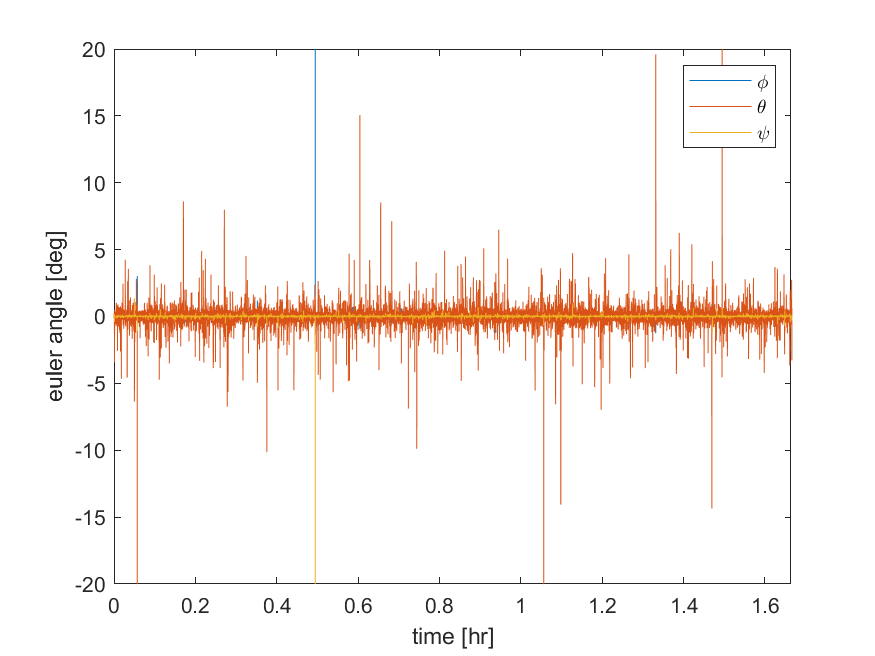
\includegraphics[scale=0.6]{Images/ps7_problem2_DADFict.png}
\caption{Attitude error using deterministic attitude determination}
\label{fig:ps7_problem2_DADFict}
\end{figure}

\begin{figure}[H]
\centering
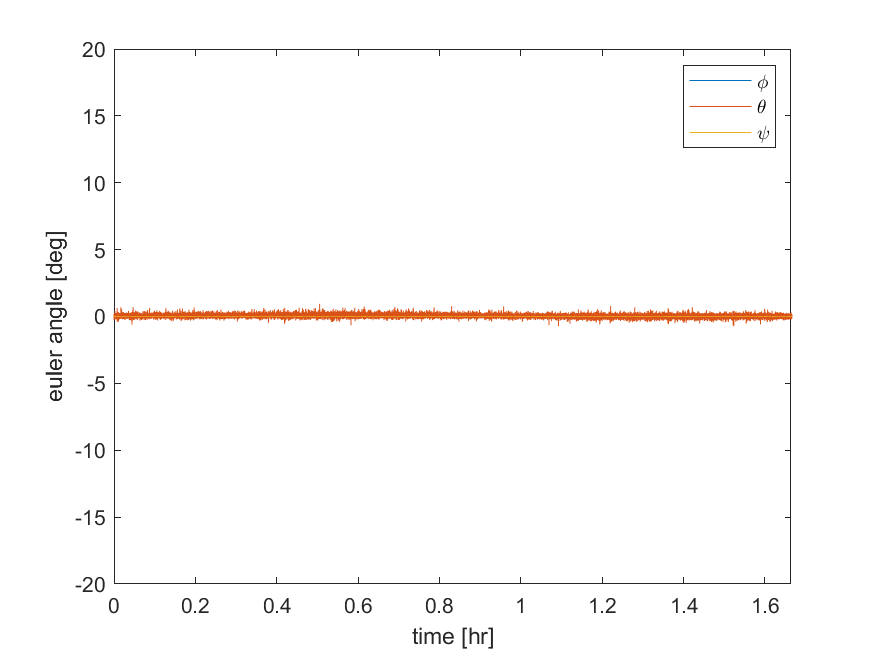
\includegraphics[scale=0.6]{Images/ps7_problem2_qMethod.png}
\caption{Attitude error using q Method}
\label{fig:ps7_problem2_qMethod}
\end{figure}

\begin{figure}[H]
\centering
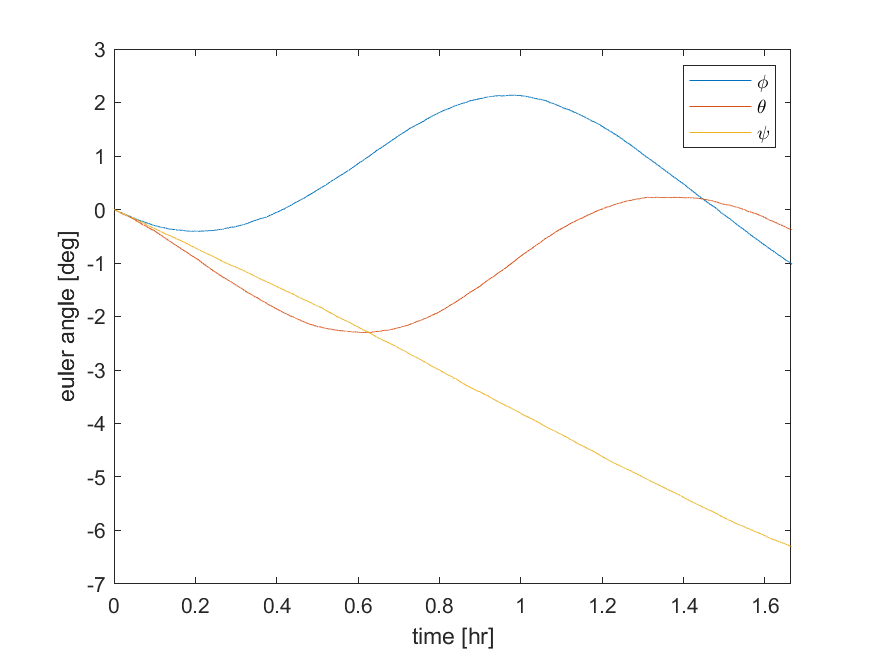
\includegraphics[scale=0.6]{Images/ps7_problem2_kin.png}
\caption{Attitude error using kinematic attitude determination}
\label{fig:ps7_problem2_kin}
\end{figure}

\subsection{PROBLEM 3}
\textit{For small sensor errors, the DCM corresponds to a small rotation. Can you give an interpretation of small angles (e.g., in Euler angles and quaternions) to the obtained error DCM?}

\subsection{PROBLEM 4}
\textit{Start modeling actual sensors in dedicated (Simulink or otherwise) subsystems which are part of the spacecraft. These models take inputs from ground-truth simulation and provides output measurements, including systematic and random errors. Take inspiration from overview of sensors discussed in class and textbook for typical errors.}

\subsection{PROBLEM 5}
\textit{Designing and implement the time update of a KF/EKF to obtain the best estimate of the state from the available measurements and models:}

The following MATLAB function is our time update-only implementation of a multiplicative extended Kalman filter (MEKF). We describe the formulation of the MEKF immediately following this function.

\lstinputlisting{src/timeUpdate.m}

\textit{Search in literature, define, and code a state transition matrix $\Phi$ which provides your state at step k+1 based on the state at step k. Verify that the output of this propagation step is consistent with the rigorous propagation of the attitude (numerical integration). Plot propagation errors as needed.}

Our state consists of 3 small angles (zero mean) and angular velocities. Our state does not track the attitude directly, but we can compute quaternions using known kinematics.
\begin{align*}
    \Vec{x} = \begin{bmatrix}
        \alpha_{x} & \alpha_{y} & \alpha_{z} & \omega_{x} & \omega_{y} & \omega{z}
    \end{bmatrix}^{\intercal}
\end{align*}

The small angle component of our state is reset every iteration and not updated in the time update step \cite{CubeSatTelescope}.
\begin{align*}
    A &= I_{3} + \frac{s_{\omega}}{\omega} [\Vec{\omega}_{t} \times] + \frac{1 - c_{\omega}}{\omega^{2}} [\Vec{\omega}_{t} \times] [\Vec{\omega}_{t} \times] \\
    \Phi_{\omega} & = I_{3} + \Delta t \begin{bmatrix}
        0 & \frac{I_{y} - I_{z}}{I_x} \omega_{z_{t}} & \frac{I_{y} - I_{z}}{I_x} \omega_{y_{t}} \\
        \frac{I_{z} - I_{x}}{I_y} \omega_{z_{t}} & 0 & \frac{I_{z} - I_{x}}{I_y} \omega_{x_{t}} \\
        \frac{I_{x} - I_{y}}{I_z} \omega_{y_{t}} & \frac{I_{x} - I_{y}}{I_z} \omega_{x_{t}} & 0
    \end{bmatrix} \\
    \Phi &= \begin{bmatrix}
        A & 0 \\
        0 & \Phi_{\omega}
    \end{bmatrix}
\end{align*}

Since we are using a MEKF, we propagate the quaternion attitude representation outside of the state vector. The quaternion attitude is propagated by $\Omega (\Vec{\omega})$, identical to the quaternion kinematics used previously.

We plot the attitude from our MEKF and our numerical integration simulation, respectively. Upon inspection, these plots appear identical. Small errors in the simulation are analyzed later in Problem 6.

\begin{figure}[H]
\centering
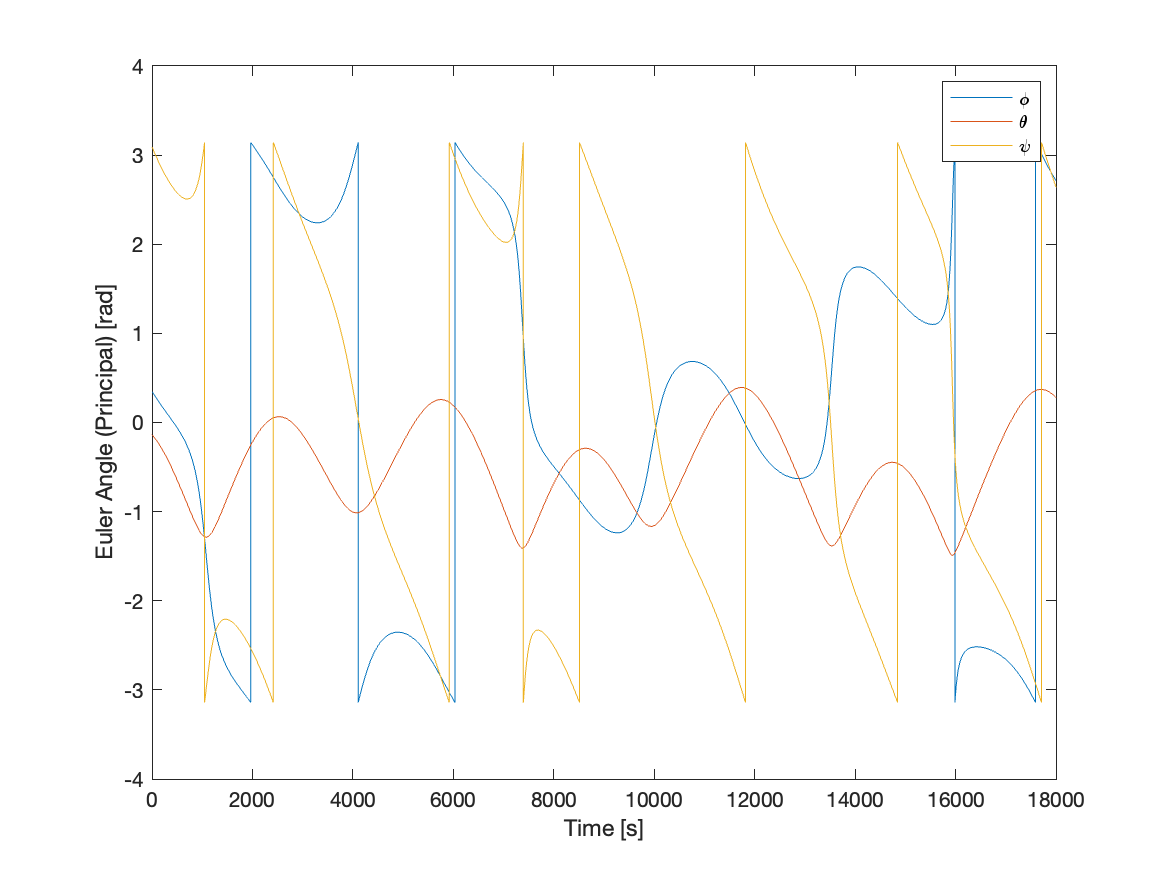
\includegraphics[scale=0.6]{Images/ps7_problem5a_angle_est.png}
\caption{Attitude evolution based on MEKF time update}
\label{fig:ps7_problem5a_angle_est}
\end{figure}

\begin{figure}[H]
\centering
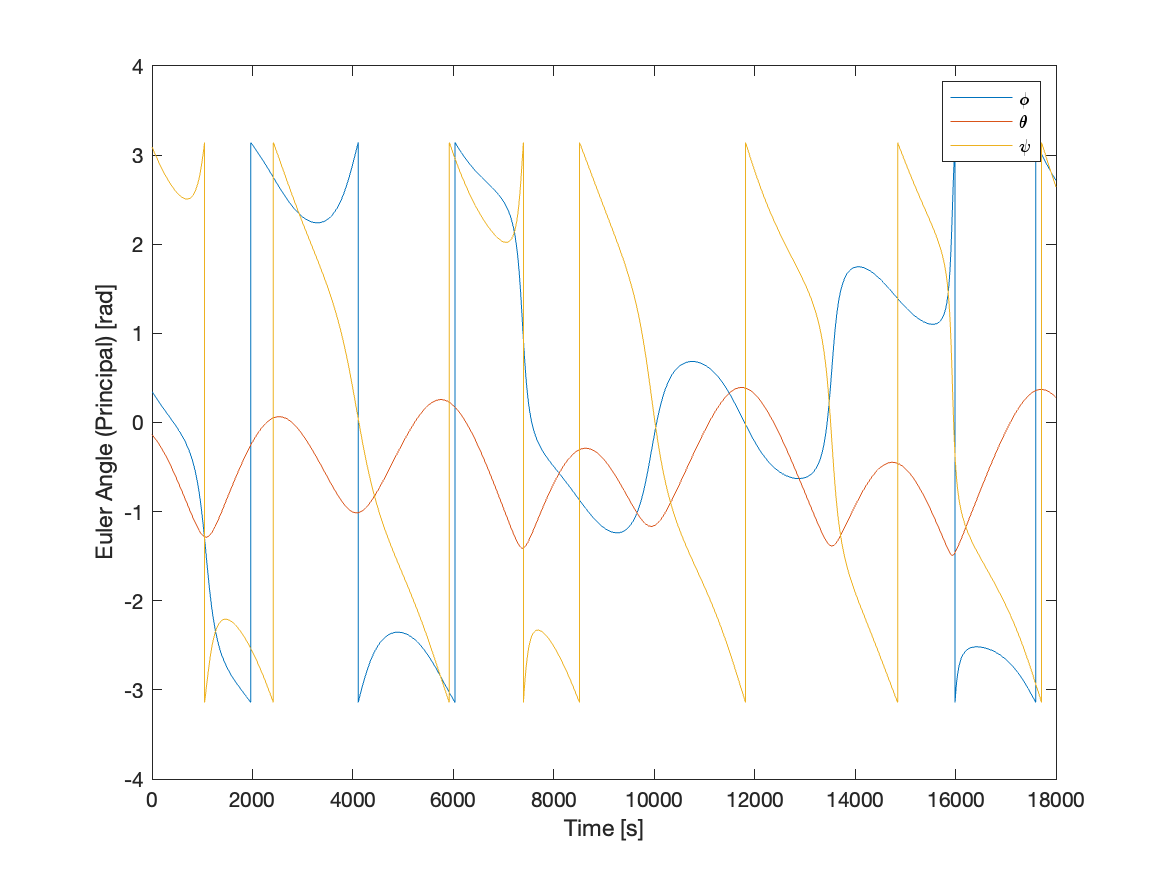
\includegraphics[scale=0.6]{Images/ps7_problem5a_angle_sim.png}
\caption{Attitude evolution from "ground truth" simulation}
\label{fig:ps7_problem5a_angle_sim}
\end{figure}

We also plot the angular velocity from both the MEKF time update step and the numerical simulation. As with the attitude evolution, both plots appear to be the same. Note that we do not include perturbations in our simulation in our comparison, as the state would quickly diverge otherwise because the measurement update is not yet implemented in the MEKF.

\begin{figure}[H]
\centering
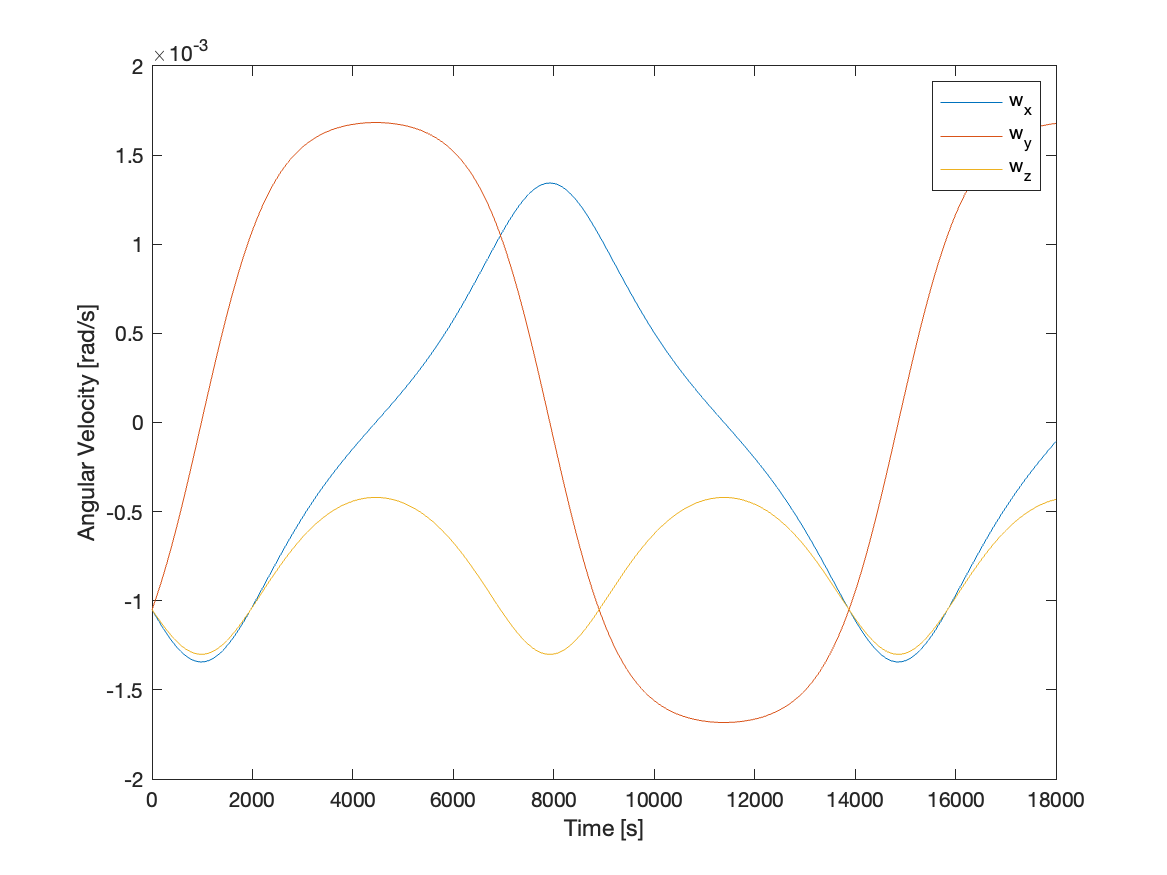
\includegraphics[scale=0.6]{Images/ps7_problem5a_angvel_est.png}
\caption{Angular velocity based on MEKF time update}
\label{fig:ps7_problem5a_angvel_est}
\end{figure}

\begin{figure}[H]
\centering
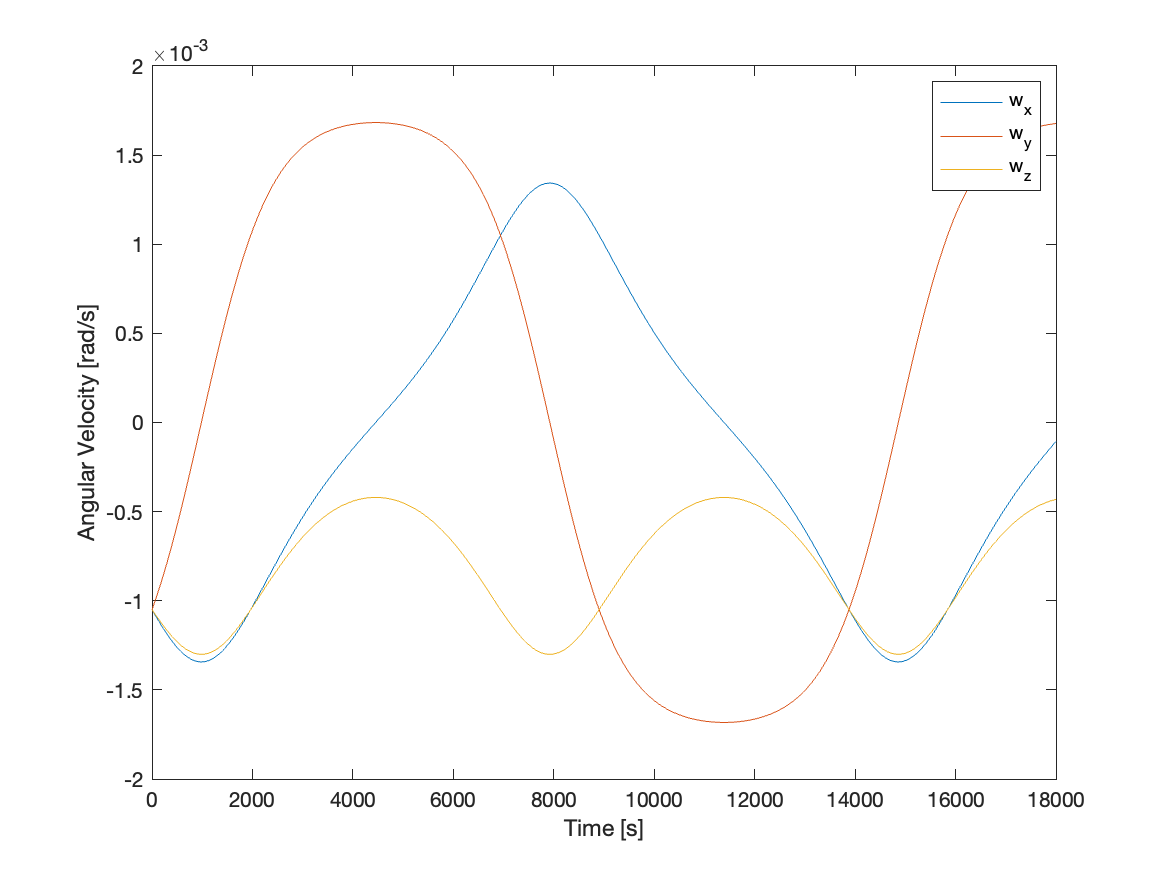
\includegraphics[scale=0.6]{Images/ps7_problem5a_angvel_sim.png}
\caption{Angular velocity from "ground truth" simulation}
\label{fig:ps7_problem5a_angvel_sim}
\end{figure}

\textit{Search in literature, define, and code a control input matrix B which provides the increment to your state at step k+1 due to a control torque at step k. Hint: optional at this stage since you do not have a controller yet.}

For now, we choose to model our control inputs as torque inputs (moments) about the principal axes. Thus, we can choose a $B$ matrix as follows:
\begin{align*}
    u_{t} &= \begin{bmatrix}
        M_{x_{t}} & M_{y_{t}} & M_{z_{t}}
    \end{bmatrix} \\
    B &= \Delta t \begin{bmatrix}
        \frac{1}{I_{x}} & 0 & 0 \\
        0 & \frac{1}{I_{y}} & 0 \\
        0 & 0 & \frac{1}{I_{z}}
    \end{bmatrix}
\end{align*}

\textit{(a) and (b) allow you to propagate the state from k to k+1 including the known control input torques. Hint: Initially you will design the filter by neglecting any control torque from your simulation.}

We have not yet implemented a controller at this step. As such, we will run the MEKF with $u_{t} = 0$ for now.

\textit{Define and code an initial state error covariance matrix P which quantifies the uncertainty of your initial state. This can be picked as diagonal matrix with diagonal elements representing the variance of each state parameter $\sigma^{2}$. Initially you can neglect cross-covariance terms assuming that errors of various state components are not correlated.}

We set our initial state error covariance matrix $P$ as a diagonal matrix, with the diagonal entries corresponding to $\alpha$ set to $1$ and the entries corresponding to $\omega$ to the variance computed from th angular velocity in the 

\textit{The time update of the EKF needs $\Phi$, B, and P. Hint: You could increment your navigation performance by keeping the filter receptive to new measurements at steady state through the addition of constant process noise Q at each step. Initially you can define Q similar to P but much smaller (e.g., 1/10 or 1/100).}

For the purpose of this section, we arbitrarily define $Q = P_{t=0} \times 0.01$.

\subsection{PROBLEM 6}
\textit{Produce plots showing true attitude estimation errors (estimate vs truth with statistics), formal or estimated attitude estimation errors (covariance from filter). Discuss the results, do they meet expectations? How well is the true estimation error described by the formal covariance? Note that we are only implementing the time update even if we call them “attitude estimates and estimation errors”.}

\begin{figure}[H]
\centering
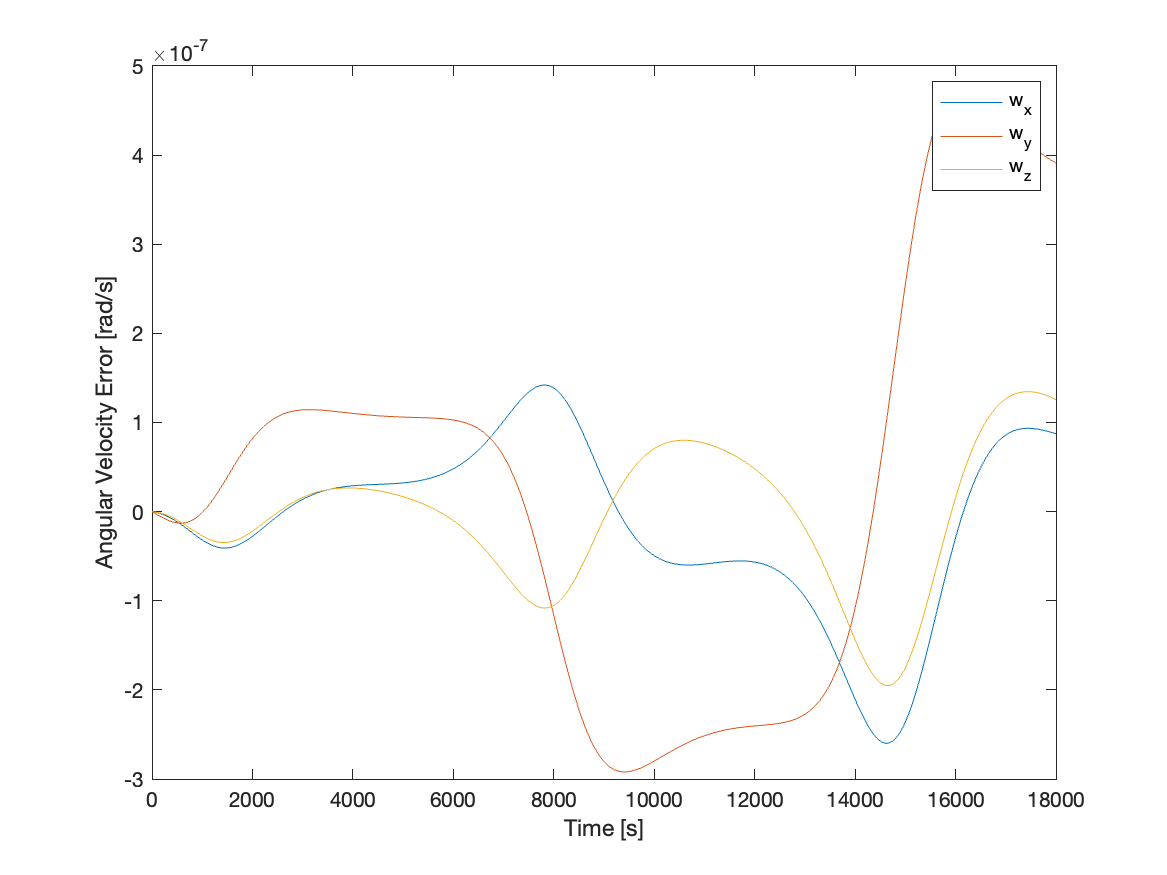
\includegraphics[scale=0.6]{Images/ps7_problem6_angvel_err.png}
\caption{Attitude error between estimate and simulation}
\label{fig:ps7_problem5a_angvel_sim}
\end{figure}

\begin{figure}[H]
\centering
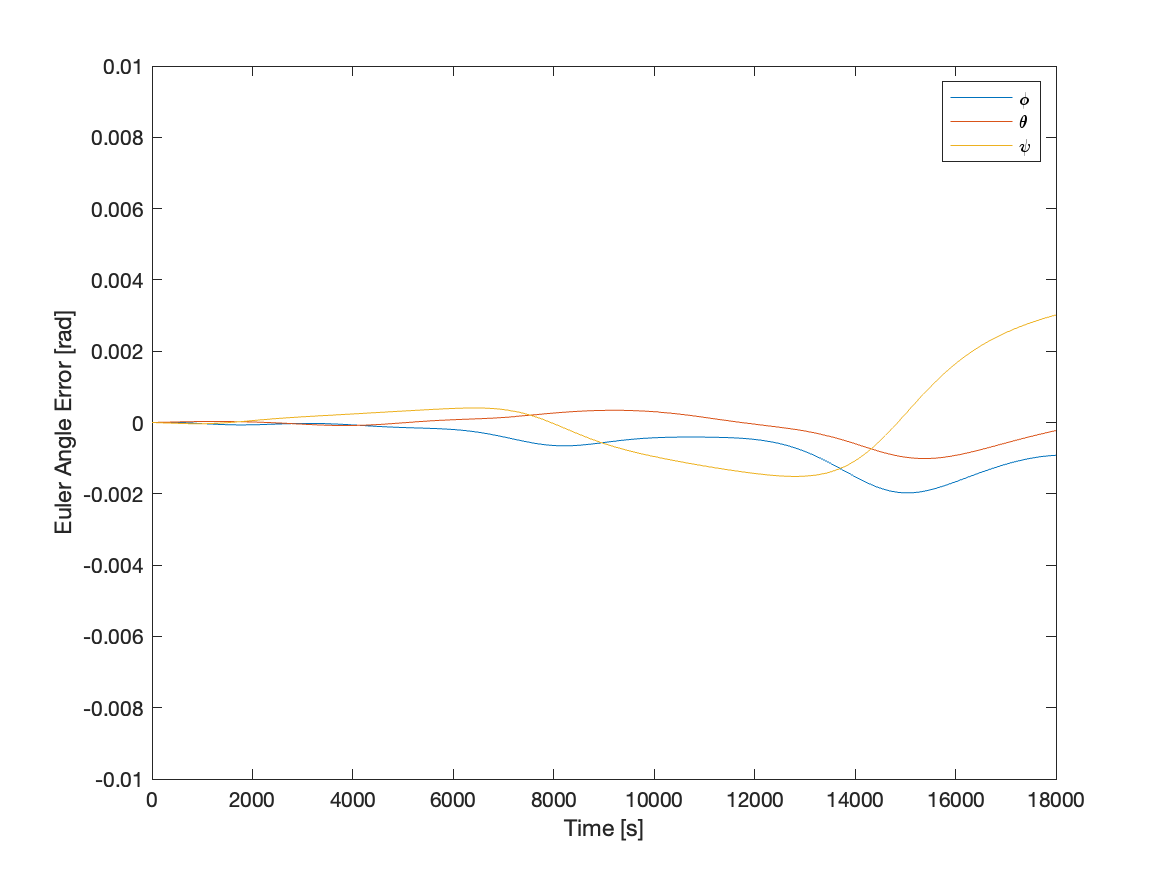
\includegraphics[scale=0.6]{Images/ps7_problem6_angle_err.png}
\caption{Angular velocity error between estimate and simulation}
\label{fig:ps7_problem5a_angvel_sim}
\end{figure}